\section{Pregunta N$^{\circ}$7\qquad Andre Gilmer Santos Felix}

\begin{frame}
	\begin{enumerate}\setcounter{enumi}{6}
		\item

		      Encuentre el interpolante de Lagrange
		      \begin{math}
			      p_{3}\left(t\right)=
			      \sum\limits_{k=0}^{3}
			      x_{k}
			      \ell_{k}\left(t\right)
		      \end{math}
		      para el conjunto de datos
		      \begin{math}
			      \left\{
			      \left(0,1\right),
			      \left(\frac{1}{2},2\right),
			      \left((1,\frac{3}{2}\right),
			      \left((2,-1\right)
			      \right\}
		      \end{math}.
		      Encuentre $p_{2,k}$ en
		      \begin{math}
			      p_{3}\left(t\right)=
			      \sum\limits_{k=0}^{3}
			      p_{3,k}t^{k}
		      \end{math}.
	\end{enumerate}

	\begin{solution}
		\begin{align*}
			\ell_{0}\left(t\right) & =
			\prod\limits_{\substack{j=0                                   \\j\neq 0}}^{n}
			\dfrac{t-t_{j}}{t_{0}-t_{j}}=
			\dfrac{\left(t-t_{1}\right)\left(t-t_{2}\right)\left(t-t_{3}\right)}{\left(t_{0}-t_{1}\right)\left(t_{0}-t_{2}\right)\left(t_{0}-t_{3}\right)}=
			\dfrac{\left(t-\dfrac{1}{2}\right)\left(t-1\right)\left(t-2\right)}{\left(0-\dfrac{1}{2}\right)\left(0-1\right)\left(0-2\right)}=
			-\left(t-\dfrac{1}{2}\right)\left(t-2\right)\left(t-1\right). \\
			\ell_{1}\left(t\right) & =
			\prod\limits_{\substack{j=0                                   \\j\neq 1}}^{n}
			\dfrac{t-t_{j}}{t_{1}-t_{j}}=
			\dfrac{\left(t-t_{0}\right)\left(t-t_{2}\right)\left(t-t_{3}\right)}{\left(t_{1}-t_{0}\right)\left(t_{1}-t_{2}\right)\left(t_{1}-t_{3}\right)}=
			\dfrac{\left(t-0\right)\left(t-1\right)\left(t-2\right)}{\left(\dfrac{1}{2}-0\right)\left(\dfrac{1}{2}-1\right)\left(\dfrac{1}{2}-2\right)}=
			2.66666666666667t\left(t-2\right)\left(t-1\right).            \\
			\ell_{2}\left(t\right) & =
			\prod\limits_{\substack{j=0                                   \\j\neq 2}}^{n}
			\dfrac{t-t_{j}}{t_{2}-t_{j}}=
			\dfrac{\left(t-t_{0}\right)\left(t-t_{1}\right)\left(t-t_{3}\right)}{\left(t_{2}-t_{0}\right)\left(t_{2}-t_{1}\right)\left(t_{2}-t_{3}\right)}=
			\dfrac{\left(t-0\right)\left(t-\dfrac{1}{2}\right)\left(t-2\right)}{\left(1-0\right)\left(1-\dfrac{1}{2}\right)\left(1-2\right)}=
			-2x(x - 2)(x - 0.5).                                          \\
			\ell_{3}\left(t\right) & =
			\prod\limits_{\substack{j=0                                   \\j\neq 3}}^{n}
			\dfrac{t-t_{j}}{t_{3}-t_{j}}=
			\dfrac{\left(t-t_{0}\right)\left(t-t_{1}\right)\left(t-t_{2}\right)}{\left(t_{3}-t_{0}\right)\left(t_{3}-t_{1}\right)\left(t_{3}-t_{2}\right)}=
			\dfrac{\left(t-0\right)\left(t-\dfrac{1}{2}\right)\left(t-1\right)}{\left(2-0\right)\left(2-\dfrac{1}{2}\right)\left(2-1\right)}=
			0.333333333333333x(x - 1)(x - 0.5).
			\shortintertext{Entonces,}
			p_{3}\left(t\right)    & =
			\sum\limits_{k=0}^{3}
			x_{k}
			\ell_{k}\left(t\right)=
			\alert{x_{0}}\ell_{0}\left(t\right)+
			\alert{x_{1}}\ell_{1}\left(t\right)+
			\alert{x_{2}}\ell_{2}\left(t\right)+
			\alert{x_{3}}\ell_{3}\left(t\right)=
			\ell_{0}\left(t\right)+
			2\ell_{1}\left(t\right)+
			\dfrac{3}{2}\ell_{2}\left(t\right)-
			\ell_{3}\left(t\right).                                       \\
			                       & =
			\alert{0}+
			2\alert{0}-
			\dfrac{3}{2}\alert{0}-
			\alert{0}=
			0.
		\end{align*}
	\end{solution}
\end{frame}

% \begin{frame}
% 	\begin{solution}
% 		\begin{figure}[ht!]
% 			\centering
% 			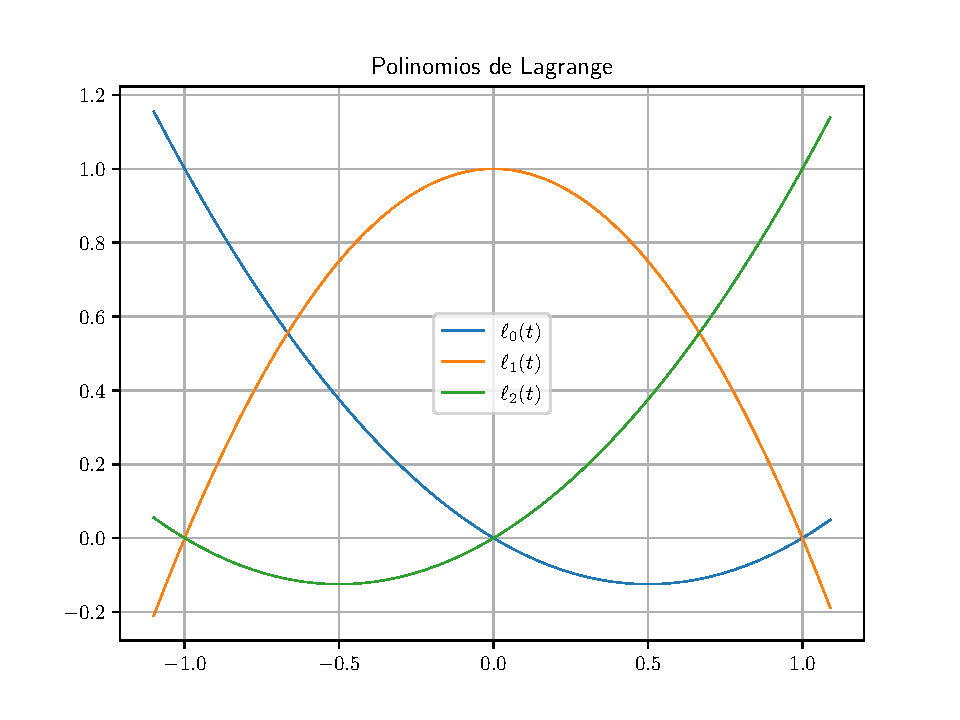
\includegraphics[width=.8\paperwidth]{p6_lagrange}
% 		\end{figure}
% 	\end{solution}
% \end{frame}

\begin{frame}
	\begin{solution}
		\begin{figure}[ht!]
			\centering
			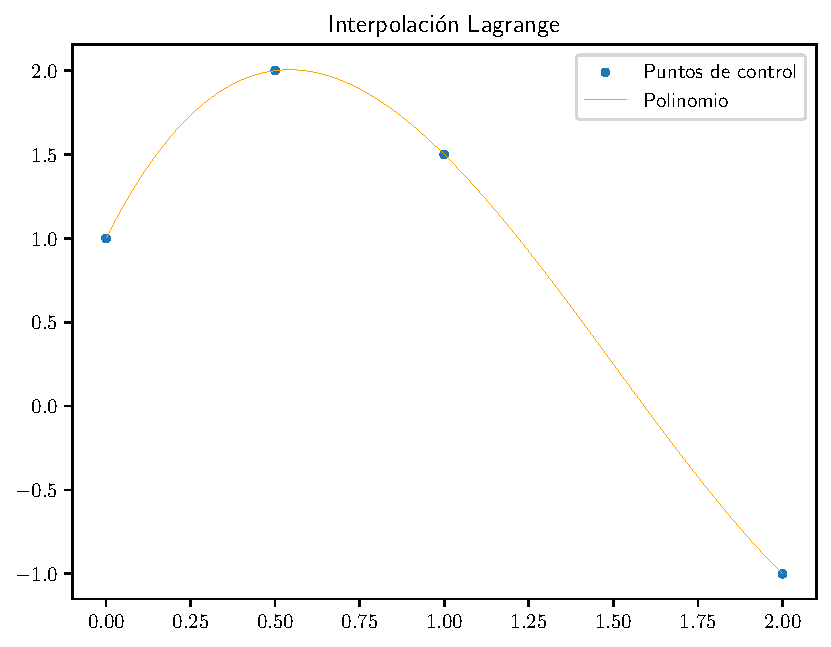
\includegraphics[width=.72\paperwidth]{p7}
		\end{figure}
	\end{solution}
\end{frame}